% Software Frontend (HTML/CSS/JS; Vue.js)
% Zuständig: Arthur

\chapter{Software - Frontend}
\label{sec:software_frontend}
Das Frontend wurde als Webanwendung realisiert,
welche die vom Server gesammelten Daten visualisiert.
%
Dazu zählen z.B. die Daten vom LiDAR-Sensor,
vom Beschleunigungssensor
und die Geschwindigkeit der Roboter,
welche mithilfe der Encoder ausgelesen wird.
%
Um die Aktivitäten der Roboter mitverfolgen zu können,
ohne vor Ort anwesend sein zu müssen,
werden auch die Livestreams von Kameras,
welche auf den Robotern angebracht sind,
angezeigt.

Das Frontend wird mithilfe von Vue.js programmiert.
%
Vue.js ist ein JavaScript-Framework zur Webentwicklung
und bietet verschiedene Möglichkeiten,
Webseiten zu programmieren.
%
Bei Vue.js kann man zwischen der ``Options'' oder
der neueren ``Composition'' API unterscheiden.
%
Die Composition API ist etwas flexibler in der Anwendung,
während die Options API eine klar definierte Struktur verfolgt.
%
Letztlich ist es dem Entwickler überlassen,
je nach seinen Präferenzen zu wählen.
%
Wir verwenden für unsere Anwendung die Composition API,
da diese etwas intuitiver ist
und ``normalem'' JavaScript etwas näher kommt. 
%
Der große Vorteil des Vue.js Frameworks ist,
dass man einzelne Komponenten einer Website
als sogenannte SFC\footnote{Single-File Components}s definiert.
%
Wie der Name schon impliziert ist in diesem SFC alles enthalten,
was diese Komponente braucht: HTML, CSS und Type-/JavaScript.
%
Dadurch wird der Code schön strukturiert und klar aufgeteilt.
%
Des Weiteren können Vue-Komponenten auch
in anderen Komponenten wiederverwendet werden,
was eine schöne Abstrahierung ermöglicht.

\section{Webseite}
\label{subsec:frontend_Webseite}
Nach der Einführung des Frontendes in Kapitel \ref{sec:software_frontend} folgt eine detaillierte
Beschreibung der Webseite sowie ihrer Funktionen. 
%
Wie bereits erwähnt, dient die Webseite der Veranschaulichung 
und bearbeitung der Daten die vom Server empfangen werden. 
%
Diese Daten werden als rohe Binärwerte empfangen und dann im Code der Webseite,
genauer im Modul ``websockets.vue'' deserialisiert werden. 
Das Deserialisieren stellt sicher, dass die übertragenen Informationen in einer für den Benutzer 
verständlichen und brauchbaren Form bereitgestellt werden. 
%
Das Hauptziel der Webseite ist es, die empfangenenen Daten des Servers in brauchbare Werte umzuwandeln. 
Diese umgewandelten Daten werden dann für weitere Berechnungen verwendet sodass eine sinvolle grafische Darstellung
erstellt werden kann.
%
Die grafische Darstellung der verschiedenen unterteilten Sensorwerte ermöglicht dem Nutzer Muster sowie 
Zusammenhänge zu erkennen. 
%
Die grafische Darstellung soll für jeden Sensor unterschiedlich erfolgen. So können potentielle Schwierigkeiten 
der Roboter grafisch analysiert werden. Dies kann beim interpretieren helfen und zukünftige Fehler vorbeugen. 
%
Nicht nur sollen die Daten angezeigt werden, dass wichtigste ist es die empfangen Daten 
in Echtzeit anzeigen zu lassen, sodass stets die neusten und aktuellsten Informationen präsentiert werden können.
%
Die Webseite ist so aufgebaut, dass sofern ein weitere Sensor implementiert werden sollte, 
der Code mit leichtigkeid erweiter werden kann und es zu keinen weiteren Schwierigkeiten kommen kann.  

\section{LiDAR-Karte}
\label{subsec:frontend_lidar_map}
Die LiDAR-Karte wird mithilfe von Vue.js auf dem Frontend,
der Webseite,
generiert und soll Hindernisse wie Wände,
Säulen oder auch Menschen mit farbigen Punkten anzeigen.
%
Hierbei gibt es aber keine Klassifikation des Hindernistyps,
abgesehen von der Erkennung von Tamerlan und Bambi.
%
Neben der verschiedenen Hindernisse,
die auf der Karte einzusehen sind,
sollen auch die Position der Roboter markiert werden.

\begin{figure}[H]
    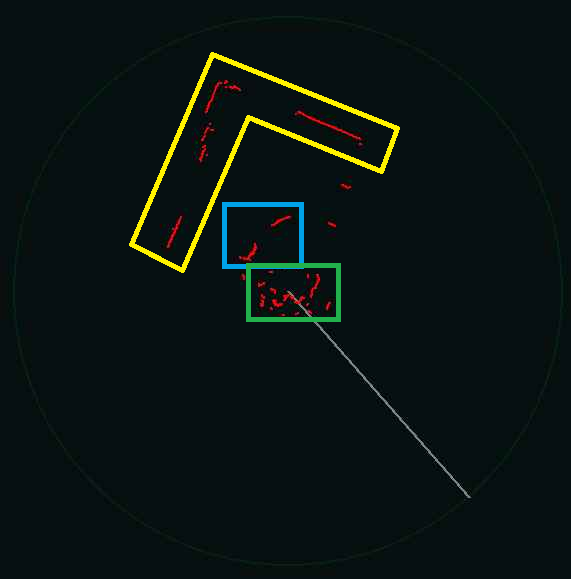
\includegraphics[width=0.7\textwidth, center]{img/LiDARMessungZeichnung_alt.png}
    \caption{LiDAR-Messung}
    \label{fig:LiDAR-Messung}
\end{figure}

Das Bild zeigt die generierte Punktwolke des LiDAR-Sensors.
%
Die Punktwolke zeigt ideal die Funktionsweise des LiDARs
und ist leicht zu interpretieren.
%
Die unterschiedlichen Laserimpulse,
welche gesendet werden,
reflektieren an der Oberfläche und werden gemessen.
% TODO @Arthur was hast du da gemeint???
Nicht nur ist die Entfernung, sondern auch die Tiefenwahrnehmung somit feststellbar.

Zur einfacheren Interpretation des Beispiels
wurden von Herrn Burjak Bereiche eingezeichnet:
%
Der grüne Bereich zeigt Objekte,
welche unmittelbar vor dem LiDAR standen.
%
In dem Fall waren es Büromaterialien wie etwa Kugelschreiber, Hefte, etc.
%
Blau markiert ist eine Person (links),
die ungefähr in 2.5 m Entfernung vom Sensor
neben einem Sessel (rechts) steht.
%
Im gelbem ``L'' kann man die Wände bzw. Bücherregale erkennen,
welche den Testraum abgegrenzt haben.
Die beiden großen Lücken im gelbem Bereich wurden
durch die Hindernisse im blauem Bereich verursacht,
an denen der Laser bereits schon frühzeitig abgeprallt ist.
%
Die beiden nicht markierten Punkte-``Cluster'' stellen Dachstützen dar.

\section{Anzeigen der Sensordaten}
\label{subsec:frontend_sensors}
Die Sensordaten werden alle auf dem Frontend dargestellt und stetig aktualisiert.
%
Jeder Tumbller-Roboter ist ab Werk mit Beschleunigungssensoren und Drehgebern ausgerüstet,
welche wir gleich für unsere Zwecke wiederverwendet haben.
%
Als Modifikationen haben wir jedem Roboter ein Kompass-Modul
und Guide zusätzlich noch den LiDAR installiert.
%
Der LiDAR erstellt eine Karte in Form einer Punktwolke,
um eventuelle Hindernisse erkennen zu können.
%
Für mehr Informationen zum LiDAR-Sensor siehe Abschnitt \ref{subsec:ueberblick_lidar} oder \ref{subsec:frontend_lidar_map}.

\begin{figure}[H]
    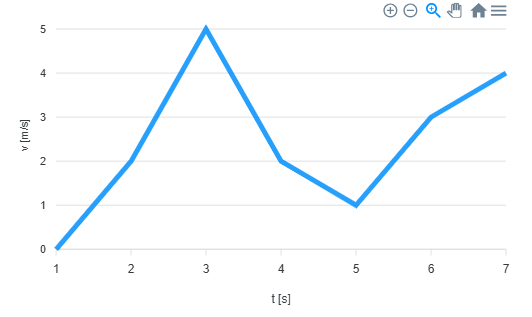
\includegraphics[width=0.8\textwidth, center]{img/encoder_chart.png}
    \caption{Diagramm der Encoderdaten}
    \label{fig:Encoderdaten}
\end{figure}

Die Werte der Beschleunigungssensoren werden,
im Graphen abhängig von der Zeit angezeigt, 
um die aktuellen Werte mit der Vergangenheit vergleichen zu können.

\section{Fernüberwachung per Kamera}
\label{subsec:frontend_cam_stream}
Auf allen drei Robotern befinden sich fest montierte
\texttt{ESP32-CAM}-Kameramodule zur Überwachung,
welche dem Frontend via MJPEG ein Live-Bild bereitstellen.
%
Die Kameras dienen vor allem der Überwachung der Roboter und sollen der Gruppe nur helfen,
mögliche Probleme (z.B. Stiegen) rasch zu identifizieren,
um die Sicherheit der Roboter zu gewährleisten.
%
Eingriffe erfolgen nur falls die Roboter nicht selbstständig erfolgreich die Gefahrensituation vermeiden.
%
Sollte ein Fehler bei der autonomen Steuerung von einem der Roboter aufgetreten sein,
helfen uns die Kameras zusätzlich bei der manuellen Fernsteuerung.
%
So können wir mithilfe der Fernsteuerung (Siehe Abschnitt \ref{subsec:frontend_control}) probieren,
die Roboter z.B. aus einer Gefahrenzone zu entfernen.

\section{Fernsteuerung}
\label{subsec:frontend_control}
Das Konzept der Fernsteuerung wurde aus den Prototypen der Projektwoche aus dem Jahr 2023/2024 übernommen.
%
Diese hatten eine Fernsteuerungsfunktion per Playstation 4 Controller. Einfachkeitshalber wurden die Roboter über 
den Laptop mittels Playstation 4-Controller angesteuert. 
%
Das größte Problem der Playstation 4-Controller besteht darin, dass sie jedes mal ihre MAC-Adresse ändern sofern
man sie über die Roboter verbindet.  
%
Die Fernsteuerungsfunktion sollte aber nur zu Testzwecken dienen um die Roboter 
vor potentiellen Gefahrensituation zu Retten. 

\section{Frontend - Code}
\label{subsec:frontend_Code}
Dieses Kapitel wird sich hauptsächlich mit der Beschreibung der unterschiedlichen Module des
Frontend-Codes beschäftigen. Der beschrieben Code wird mit der Methode ``4+1 architectual view model'' beschrieben.
%
Diese Methode wird bei Softwarelastigen Projekten verwendet,
um den Code auf verschieden Art und weisen zu beschreiben. 

\subsection{websocket.vue}
\label{subsec:frontend_websocket.vue}

\section{Webseitenprobleme}
\label{subsec:problem_Webseite}

\subsection{Pfadfindung}
\label{subsubsec:problem_Pfadfindung}
Um bei Vue.js Module zu importieren muss die Funktion \texttt{Import from 'PFAD'} verwendet werden.
%
Um die Encoder Daten welche vom Server geschickt werden verarbeiten zu können, 
müssen erstmals die generierten Protobufdateien gefunden werden.
%
\begin{lstlisting}[language=JavaScript,gobble=4]
  {
    import { EncoderData } from  '../lib/encoder_data'
    ...
    const decodedData = EncoderData.fromBinary(binaryData);
    ...
  }
\end{lstlisting}
Es sollte ``EncoderData`` aus der generierten TypeScript-Protobuf Datei gelesen werden und im Modul ``websocket.vue'' verwendet werden.
Dieser Ansatz wie er oben steht, führt jedoch dazu, dass der Pfad nicht gefunden wird. 
%
Nach viel Recherche viel auf, dass nicht nur JavaScript dateien generiert werden müssen, sondern auch TypeScript Dateien.
Sobald die benötigte TypeScript Datei hinzugefügt wurde, verschwand die Fehlermeldung.
%
Nachdem die vorherigen Fehlermeldungen beseitigt worden waren, kam eine neue auf. 
Der Fehler lag, daran, dass die neuen generierten Files das "google-Protobuf" Packet brauchten um zu funktionieren.
% 
\begin{lstlisting}[language=JavaScript,gobble=4]
  {
    import * as pb_1 from "google-protobuf";
    ...
  }
\end{lstlisting}
Dies war leicht zu beheben mit dem Befehl:\\ \textbf{npm install -D @types/google-protobuf} \\ wurden die Packete schnell
heruntergeladen.
